\documentclass[12pt, a4paper]{report}
\usepackage[utf8]{inputenc}
\usepackage{amsmath, amsfonts, amsthm}
\usepackage{tabularx}
\usepackage{hyperref}
\hypersetup{
    colorlinks=true,
    linkcolor=red,
    urlcolor=cyan,
    pdftitle={Facharbeit},
    }
\usepackage[ngerman]{babel}
\usepackage{xcolor}
\usepackage{geometry}
\geometry{
 a4paper,
 total={170mm,257mm},
 left=30mm,
 right=30mm,
 top=20mm,
 bottom=40mm
 }
 \usepackage{graphicx}

\usepackage[framemethod=tikz]{mdframed}

% Proposition zur korrekten Nummerierung
\newmdtheoremenv[
]{prop}{Proposition}[section]

% Spezieller Style für die Definitionen
\theoremstyle{definition}
\newmdtheoremenv[
  hidealllines=true,
  leftline=true,
  innerleftmargin=10pt,
  innerrightmargin=10pt,
  innertopmargin=0pt,
]{defi}[prop]{Definition}

% Bemerkungen Theorem
\newmdtheoremenv[
  hidealllines=true,
  innertopmargin=0pt,
]{rem}[prop]{Bemerkung}

% Korollar Theorem
\newmdtheoremenv[
  hidealllines=true,
  innertopmargin=0pt,
]{kor}[prop]{Korollar}

% Lemma Theorem
\newmdtheoremenv[
  hidealllines=true,
  innertopmargin=0pt,
]{lem}[prop]{Lemma}

\makeatletter

\newcommand*{\rom}[1]{\expandafter\@slowromancap\romannumeral #1@}
\newcommand\omicron{o}


\makeatother
\title{\LARGE   Facharbeit im Leistungskurs Mathematik  \vspace*{0.5cm} \\
  \Huge Renditenverteilung am Kapitalmarkt}
\LARGE \author{Jesse Georgias}
\LARGE \date{März 2021}

\begin{document}

\maketitle
\newpage
\vspace*{\fill}
\begin{normalsize}
\noindent
  \textbf{Satz:}
  \LaTeX
\end{normalsize}
\vspace*{5pt}
\hrule
\vspace{5pt}
\noindent
\textbf{Quellen:}
\\
Christian Limbacher, \textit{Schiefe und Kurtosis von Aktienrenditen}, Masterarbeit, Johannes Kepler Universität Linz, 2018 \\
Benoit Mandelbrot, \textit{The Variation of certain speculative Prices}, The University of Chigago Press, 1963 \\
Hanspeter Schmidli, \textit{Einführung in die Stochastik}, Vorlesungsnotizen, Universität zu Köln, 2019
\tableofcontents
\newpage
\chapter{Einleitung}
\section{Hintergrund}
Von dem Wetter über Fußballergebnisse bis zur Verspätung der Bahn, unser Alltag wird maßgeblich von Ereignissen geprägt auf die wir so gut wie keinen Einfluss nehmen können und die ebenso schwer vorherzusagen sind. Eine der interessantesten Zufallsgrößen sind die Preisentwicklung an Kapitalmärkten.
%Please work on this here%
\section{Zielsetzung}
Auf den ersten Blick sind die Vorgänge in den Finanzmärkten das reinste Chaos. Niemand kann zuverlässig vorhersagen wie sich die Märkte morgen verhalten werden. Mein Ziel ist es, in dieses Chaos Struktur zu bringen und somit dem Leser zu einem besserem Verständniss, besonders von den assoziierten Risiken, zu verhelfen. Weiterhin soll diese Arbeit aufzeigen, wie mathematische Theorien in der realen Welt Anwendung finden und somit den essenziellen Realitätsbezug eines als theoretisch wahrgenommenen Faches etablieren.

\chapter{Methodik}
\section{Datenerfassung}
In der folgenden Arbeit benutze ich einen Datensatz des sogenannten ``Standard \& Poore 500`` Indexes verwendet. Dieser umfasst die, nach Marktwert, 500 größten, öffentlichen Firmen der USA. Mit einer Marktkapitalisierung von isgesamt circa 40,2 Billion USD\footnote{Stand 31. März 2022, \href{https://www.spglobal.com/spdji/en/idsenhancedfactsheet/file.pdf?calcFrequency=M&force_download=true&hostIdentifier=48190c8c-42c4-46af-8d1a-0cd5db894797&indexId=340}{spglobal.com}} (S\&P Global, 2022, S. 5) ist dieser einer der größten nationalen Aktienindices und somit auch interessant für Untersuchungen. \\
Der Datensatz beinhaltet den monatlichen den Punktestand des Index, Dividenden, Umsatz und noch eine Reihe weiterer Datenpunkte, welche allerdings für mich nicht von Interesse sind. Da für uns die Renditen, also die prozentuale Änderung des Preises, von Interesse ist, wird die Tabelle um eine weitere Spalte ``renditen`` erweitert.
Der n-te Eintrag in Renditen ergibt sich aus den n-ten, beziehungsweise (n-1)-ten Einträgen der Punkte des S\&P 500:
\begin{center}
    $\indent r_{n} = \frac{p_{n}}{p_{n-1}} - 1 \text{ mit } n \in \mathbb{N}_{0},\ p_{n} \in \tex{ punkte,\ und \ } r_{n} \in \tex{renditen} \\$
\end{center} \\
\noindent Alle hier benutzen Daten\footnote{\url{www.econ.yale.edu/~shiller/data/ie_data.xls}}, sind Daten des Ökonomie Professors Robert Shiller, welcher diese selbst in seinen Arbeiten benutzt.
 (Irrational Exuberance, Princeton University Press 2000, Broadway Books 2001, 2nd ed., 2005)

\chapter{Die Gaussche Normalverteilung}
Da sich die meisten Zufallsgrößen und ihre Wahrscheinlichkeitsverteilung mit der gausschen Normalverteilung beschreiben lassen, wäre es ein erster Ansatz die Renditenverteilung ebenso zu modellieren.
\section{Definition einer Zufallsvariable}
Sei $\Omega$ eine abzählbare Menge\footnote{d.h., $\Omega$ ist entweder endlich, oder es gibt eine surjektive Funktion $f: \mathbb{N} \rightarrow \Omega $}, dann sind $\omega \in \Omega$ die sogenannten Elementarereignisse und $\Omega$ der sogenannte Elementarergeignissraum. \\
Ein \textbf{Ereignis} ist dann eine Teilmemge $A \subset \Omega$. Also $\mathcal{F} = \{A: A \subset \Omega \}$ ist die Klasse der Ereignisse. Wir sagen A \textbf{tritt ein}, falls ein Elementarereignis aus A eintritt.
Eine Funktion $p: \Omega \rightarrow [0, 1]$ heißt \textbf{Wahrscheinlichkeit}, falls
\begin{center}
 $ \displaystyle\sum_{\omega \in \Omega} p(\omega) &= 1 $
\end{center}
\noindent Die Abbildung
\begin{center}
    $\mathbb{P}: \mathcal{F} \rightarrow [0, 1],\ A \mapsto \displaystyle\sum_{\omega \in \Omega} p(\omega)$
\end{center}
heißt \textbf{Wahrscheinlichkeitsverteilung}. (Schmidli, \textit{Einführung in die Stochastik}, 2019, S.1 \& 2) \\
Sei $E$ ein raum wie z.B. $\mathbb{R}$, dann heißt eine Funktion $X: \Omega \rightarrow E, \omega \mapsto X(\omega)$ (E-wertige) \textbf{Zufallsvariable}\footnote{Wir schreiben $X$ wenn wir $X(\omega)$ meinen.}. $X$ ist somit ein zufälliger Wert. (Schmidli, \textit{Einführung in die Stochastik}, 2019, S.8)
\newpage

\section{Erwartungswert \& Varianz}
\subsection{Erwartungswert}
Der Erwartungswert wird wie folgt definiert:
\begin{center}
    $\mathbb{E}[X] = \displaystyle\sum_{\Omega}X(\omega)p(\omega)$
\end{center}
Bei einem Spiel stellt $X$ den Gewinn dar. Wenn wir n-mal spielen, so bekommen wir ungefähr $np(\omega)$ mal den Gewinn $X(\omega)$.
Die Summe aller Gewinne ist somit ungefähr $n\mathbb{E}[X]$, daraus folgt, dass der Erwartungswert $\mathbb{E}[X]$ ungefähr der durchschnittliche Gewinn ist.

\subsection{Varianz}
Die Varianz ist die einer Zufallsvariable $X$ ist wie folgt definiert:
\begin{center}
    $\mathbb{V}[X] = \mathbb{E}[(X- \mathbb{E}[X])^{2}] = \mathbb{E}[X^{2}] - \mathbb{E}[X]^{2}$
\end{center}
Die Varianz ist ein Strueungsmaß und gibt an, wie stark $X$ um den Erwartungswert schwankt.
Die Standardabweichung ist $\sqrt{\mathbb{V}[X]}$.

\subsection{Erwartungswert \& Varianz in empirischen Datensätzen}
Sei $X = {x_{1}, x_{2}, x_{3}, ...}$ eine endliche Menge an empirisch Beobachteten Datenpunkten der Mächtigkeit $|X|=n$. Dann ist
\begin{center}
    $\mu = \frac{1}{n}\displaystyle\sum_{i=1}^{n}x_{i}$ der Erwartungswert und $\mathbb{V}[X] = \frac{1}{n}\displaystyle\sum_{i=1}^{n}(x_{i} - \mu)^{2}$ die Varianz.
\end{center}
Die Standardabweichung $\sigma$ ergibt sich so aus $\sqrt{\mathbb{V}[X]}$.

\section{Dichte- und Verteilungsfunktion}
Die Dichtefunktion\footnote{Kurz pdf, für ``probability density function``} $f: X(\omega) \mapsto p(\omega)$ der Normalverteilung ist gegeben durch:
\begin{center}
    $ f(x) = \frac{1}{\sqrt{\sigma^{2}2\pi}}e^{-\frac{1}{2}(\frac{x-\mu}{\sigma})^{2}}
    \tex{ mit } \ \mu = \mathbb{E}[X] \text{ und } \sigma = \sqrt{\mathbb{V}[X]}$
\end{center}
\begin{figure}[htbp]
  \centering
     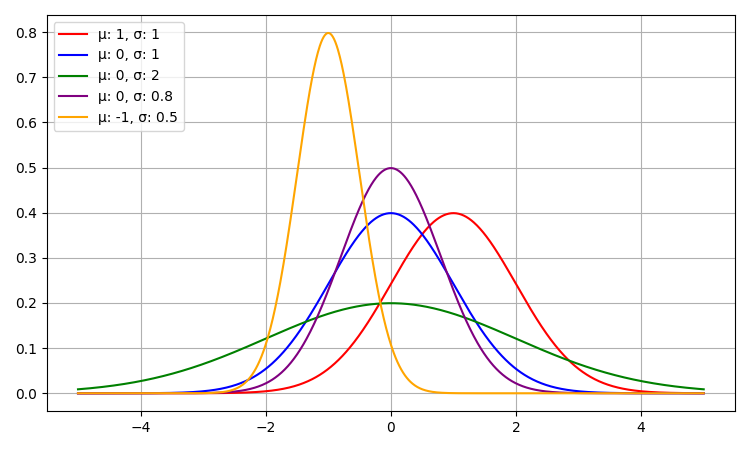
\includegraphics[width=0.8\textwidth]{bilder/N_pdf.png}
  \caption{Dichtefunktion mit unterschiedlichen Parametern}
  \label{fig:Abb.1}
\end{figure}
Da gilt $\displaystyle\sum_{\omega \in \Omega} p(\omega) &= 1 \Rightarrow \int_{-\infty}^{\infty}f(x) = 1 $ \\




\section{Die Normalverteilung als Modell für Finanzdaten}
Aus dem uns gegebenen Datensatz können ohne Probleme mithilfe der eben besprochenen Methoden, die beiden charakteristischen Momente der Normalverteilung errechnet werden. So ergibt sich für die Rendite: \\%Renditen%
$
\indent \mu  \approx 0.004439795157195 \\
\indent \sigma \approx 0.04056647568973973 \\
$
Somit kann man für den Datensatz die pdf aufstellen:
\begin{figure}[htbp]
  \centering
     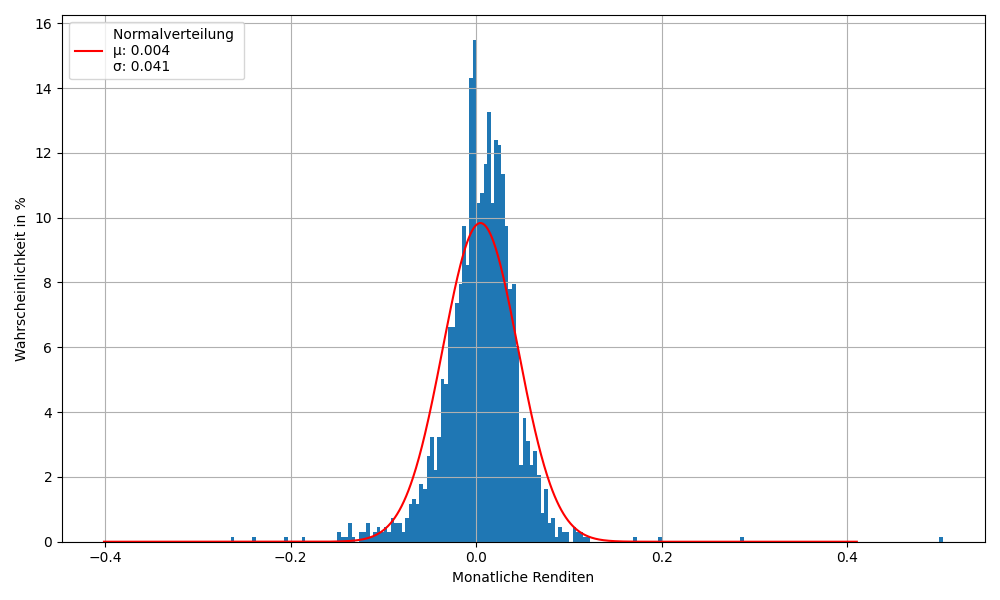
\includegraphics[width=0.9\textwidth]{bilder/N_on_returns.png}
  \caption{Dichtefunktion auf Histogram der Renditen}
  \label{fig:Abb.2}
\end{figure}

Es fällt sofort auf, dass die tatsächliche Verteilung deutlich spitzer ist als die auf die gegeben Parameter angepasste Normal Verteilung. Das heißt, dass noch deutlich mehr Wert ziemlich nahe am Erwartungswert liegen, als durch die Normalverteilung vorhergesagt. Es ist also deutlich warhrscheinlicher, dass ein wert $x$ in der nähe des Erwartungswertes liegt. Aufgrund dieser Tatsache könnte man bereits schlussfolgern, dass die Normalverteilung kein geeignetes Model ist, jedoch sind die Abweichungen nur um ein paar Prozent und man könnte dies auf einen z.B. zu kleinen Datensatz schieben.
Kritisch wird es, wenn wir uns die Häufiggkeit von Extremereignissen angucken: \\
\begin{figure}[htbp]
  \begin{center}
    \begin{tabularx}{0.5\textwidth} {
      | >{\centering\arraybackslash}X
      | >{\centering\arraybackslash}X |
       >{\centering\arraybackslash}X | }
      \hline
      Datum & Rendite (r) & $\mathbb{P}[X = r]$\\
      \hline
      1929-11-01  & -0.264737 & 2.70^{-9} \\
      \hline
      1932-04-01  & -0.239709 & 1.34^{-7}\\
      \hline
      2008-10-01  & -0.203911 & 1.84^{-5}\\
      \hline
      1932-08-01  & 0.502994 &  1.57^{-32}\\
      \hline
      1933-05-01  & 0.287373 & 2.69^{-10}\\
      \hline
    \end{tabularx}
  \end{center}
  \caption{Extremrenditen}
  \label{fig:Abb.3}
\end{figure}
\noindent
In Abb. 3.3 sind alle Monate zu sehen, in denen der S\&P500 mehr als $+20\%$ oder weniger als $-20\%$ gemacht hat und ihre enstprechenden Wahrscheinlichkeiten. Wie man sehen kann sind diese, nach der Normalverteilung, imens klein, gar fast unmöglich.
Nach dieser Modellierung würden wir es für sehr unwahrscheinlich halten, $20\%$ unseres Kapitals zu verlieren\footnote{$\mathbb{P}[X = -0.2] \approx 3 \cdot 10^{5}$} jedoch können wir genau dieses Ereigniss mehrfach beobachten.
Es sticht jedoch eine weitere Sache hervor. Im August 1932 legte der S\&P500 sage und schreibe $50\%$ zu, die assoziierte Wahrscheinlichkeit für dieses Ereigniss nach unserem Model circa $1.57^{-32}$. Dieses Ereignis sollte demnach als so gut wie unmöglich gelten, trotzdem können wir es in einem Datensatz mit nur 1780 Datenpunkten empirisch beobachten. Daraus kann man schließen, dass unser aktuelles Model unzureichend ist.
Um unsere Beobachtungen erklären zu können, bräuchten wir eine Wahrscheinlichkeitsverteilung, wo sich die Wahrscheinlichkeiten stark um das Hoch tummeln, dann jedoch nicht exponentiell abfallen, sodass die Dichtefunktion an den Rändern immernoch breit ist. "heavy-tailed"










\end{document}
